\chapter{SNAP}

El \emph{Sentinel Aplication Toolbox (SNAP)} es un  software de procesamiento de imágenes diseñado por la \emph{Agencia Espacial Europera (ESA)}, cuyas herramientas simplifican el trabajo con imágenes radar y ópticas.
Esta clase tirno vomo objetivo familiarizarce con el entorno gráfico del programa.

\section{Interfaz gráfica del SNAP}

Descomprima los archivos decargados denominanados \directory{material.tar.gz}. Abra el programa SNAP, allí encontrará la interfaz gráfica del usuario (Figura \ref{fig:int})

\begin{figure}[h!]
    \centering
    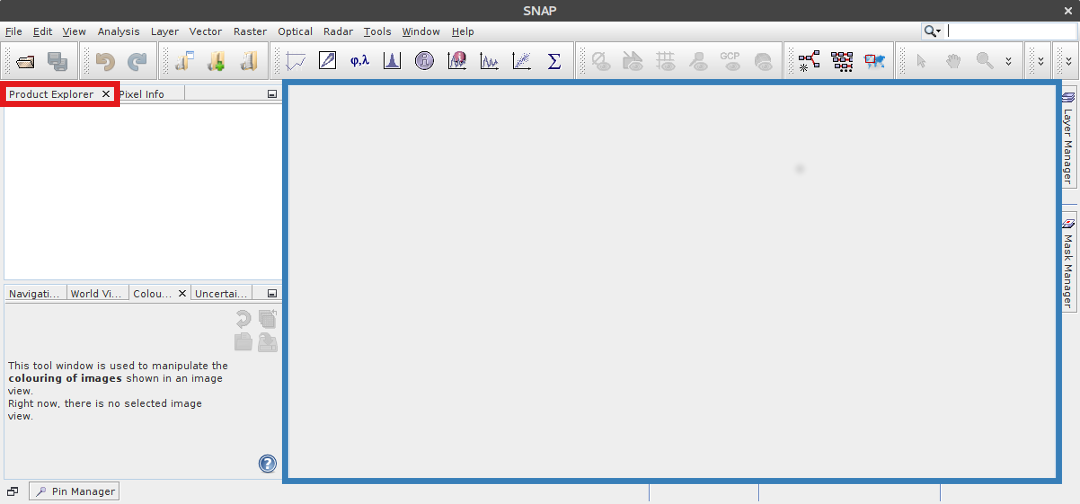
\includegraphics[scale=1.1]{fig:int.png}
    \caption{Interfáz gráfica del usuario. El area de visualización con el \emph{Producto Explorer} a la izquierda.}
    \label{fig:int}
\end{figure}

\section{Apertura de imágenes}

En el menú principal, seleccione \menu{Open product...} y dentro de la carpeta \directory{material/raster\_data}, elija \directory{S2A\_USER\_MTD\_SAFL2A\_PDMC\_20161206.dim}.

Haga doble click sobre el nombre de la imágen y se desplegará, en el \menu{Producto Explorer} un árbol que incluye las siguientes opciones:
\dirtree{%
    .1 [1] S2\_MSIL2A\_20170702.
    .2 Metadata.
    .2 Index Codings.
    .2 Vector Data.
    .2 Bands.
    .2 Masks.
}

En esta cobertura encontramos

\begin{itemize}
    \item \emph{[1] S2\_MSIL2A\_20170702}: El número de elemento entre corchetes, que marca en que orden se abrieron los productos y el nombre de la imagen.
    \item \emph{Metadata}: Los metadatos asociados a la imagen y su historial de procesamiento.
    \item \emph{Index Codings}: Los valores de referencia para interpretar los números digitales de la imagen.
    \item \emph{Vector data}: Las capas vectoriales asociadas a la imagen.
    \item \emph{Bands}: Las bandas de la imagen y las operaciones de álgebra entre bandas.
    \item \emph{Masks}: Las máscaras que sean incluidas en la imagen.
\end{itemize}

\section{Visualización}

Para visualizar una de las bandas de la imagen haga doble click sobre el nombre y se mostrará en escala de grises (Figura \ref{fig:mono}). Es posible abrir varias bandas en simultaneo, cada una se mostrará en una pestaña nueva arriba del área de visualización. Explore la imagen utilizando las herramientas de navegación y zoom (Figura \ref{fig:NAV})

\begin{figure}[h!]
    \centering
    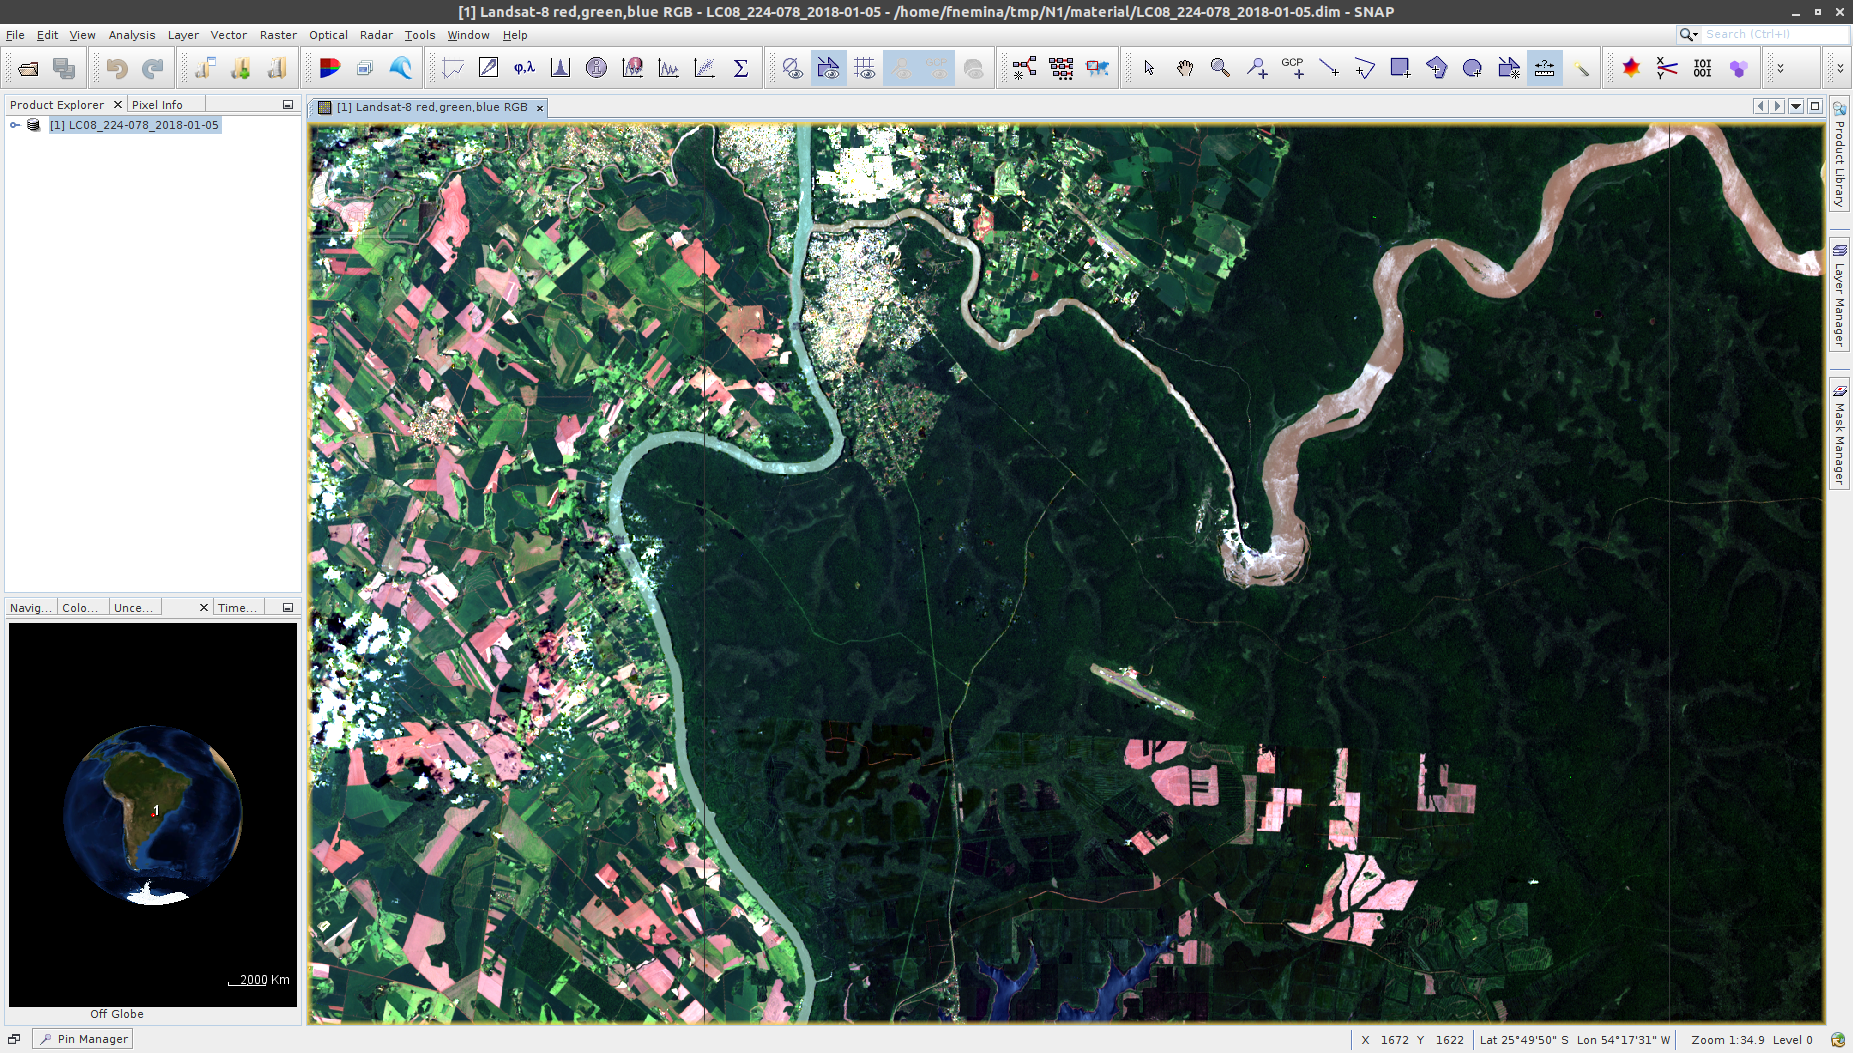
\includegraphics[scale=0.7]{fig:mono.png}
    \caption{Imagen monobanda desplegada en el visualizador.}
    \label{fig:mono}
\end{figure}



\begin{figure}[h!]
    \centering
    
\includegraphics[scale=0.5]{fig:NAV.png}
    \caption{Herramientass de navegación. De izquierda a derecha: \menu{Selection tool}, para seleccionar objetos en la imagen, \menu{Panning tool}, para moverse dentro de la imagen, y \menu{Zooming tool}, para hacer zoom en la imagen.}
    \label{fig:NAV}
\end{figure}

En el \menu{Product Explorer} haga click derecho sobre el nombre y seleccione \menu{Open RGB image windows}. Se desplegará una nueva ventana (Figura \ref{fig:RGB}) que le permitirá elegir la combinación de bandas. Por defecto aparecerá la combinación que utiliza las bandas 4, 3 y 2 de Sentinel 2, desplieguela haciendo click en OK (Figura \ref{fig:RVA}).

\begin{figure}[h!]
    \centering
    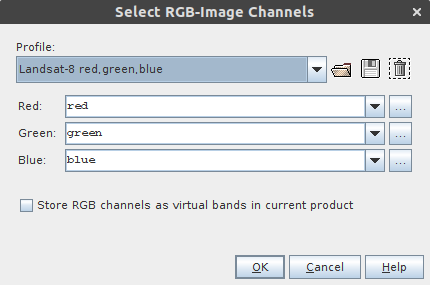
\includegraphics[scale=0.7]{fig:RGB.png}
    \caption{Ventana de combinación de bandas. Puede eligir una banda para cada canal del monitor (\emph{Red, Green, Blue}) o puede optar por una preseleccionada del menú \emph{Profile}}
    \label{fig:RGB}
\end{figure}



\begin{figure}[h!]
    \centering
    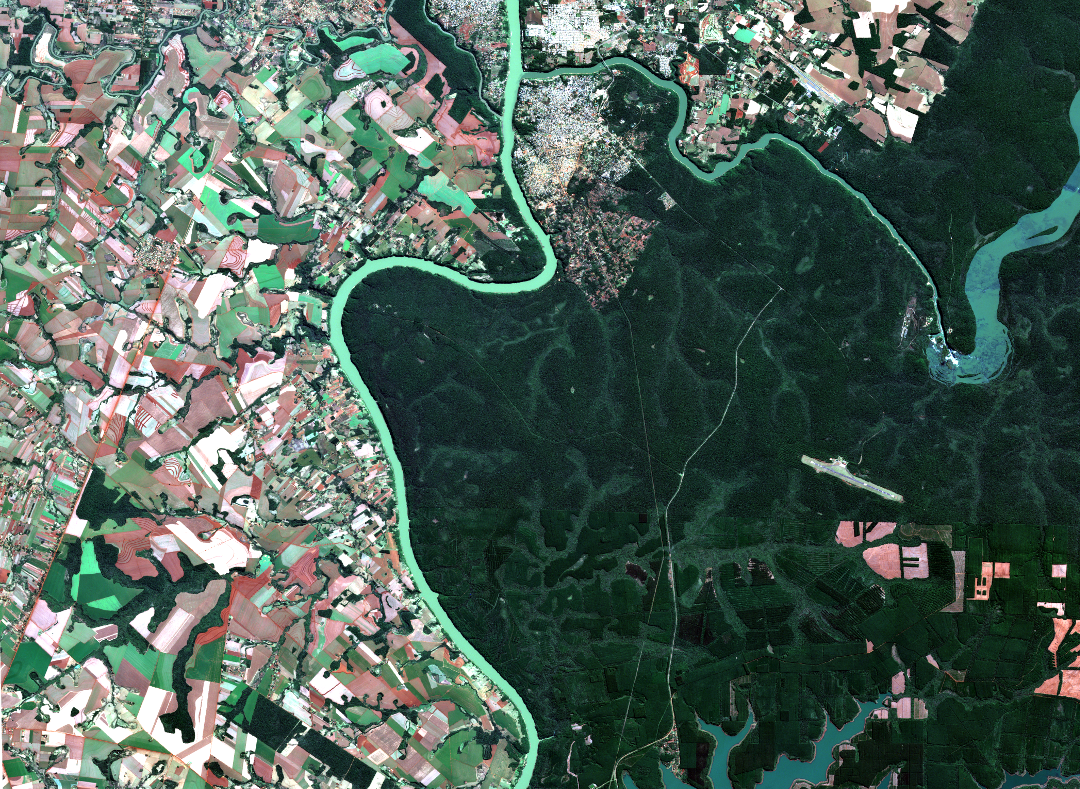
\includegraphics[scale=0.5]{fig:RVA.png}
    \caption{Imagen en combinación de colores de color real.}
    \label{fig:RVA}
\end{figure}


\section{Consulta de píxel}

Para obtener información sobre un pixel posicionese sobre uno en la imagen y seleccione la pestaña \menu{Pixel info}, junto al \menu{Product explorer} (Figura \ref{fig:pixel}).

\begin{figure}[h!]
    \centering
    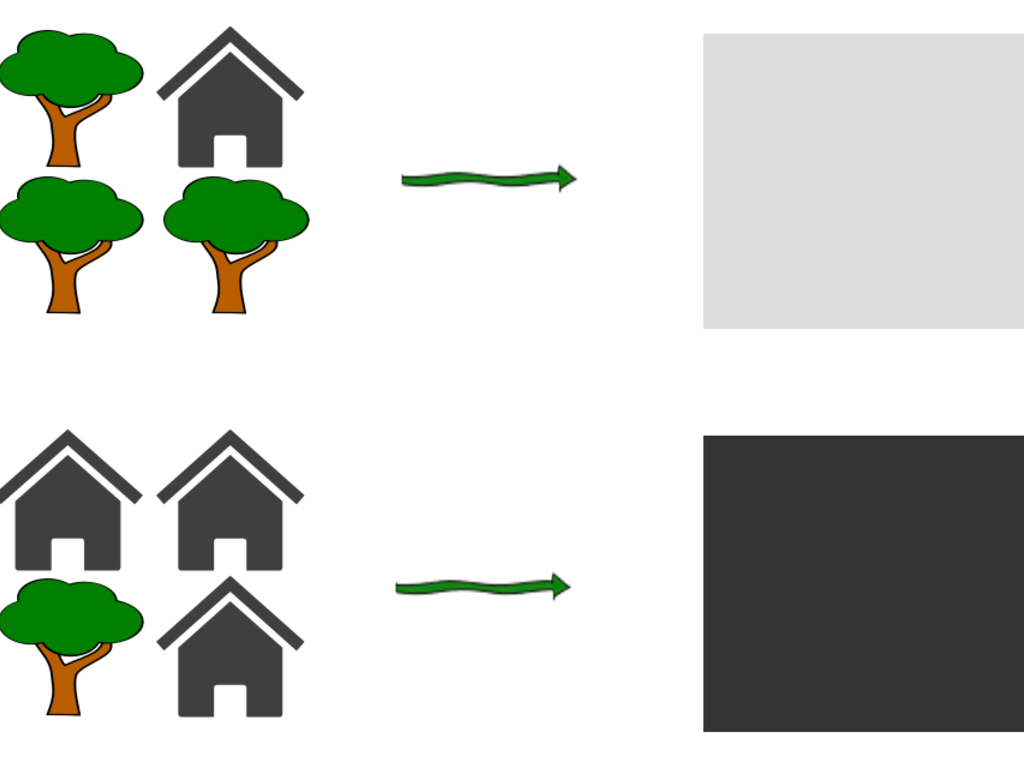
\includegraphics[width=0.3\textwidth]{fig:pixel.png}
    \caption{}
    \label{fig:pixel}
\end{figure}

Allí encontrará la latitud y longitud, las coordenadas dentro del mapa y el valor del pixel en la banda abierta.

\section{Exportar pantalla}

Es posible exportar la visualización de la imagen completa o de una región específica desde \menu{File>Export view}. Si selecciona \menu{View as KMZ} obtendrá un archivo \directory{.kmz} que luego podrá abrir desde Google Earth; o elegir \menu{View as image} generando archivos \directory{.GeoTiff} o \directory{.jpg} para visualizarlo en otro software. Para mantener la georreferencia debe optar por \emph{GeoTIFF - TIFF with geo-location} con la opción \emph{Full resolution}. De esta manera sse mantiene la resolucion original de la imagen.(Figura \ref{fig:export}).
.

\begin{figure}[h!]
    \centering
    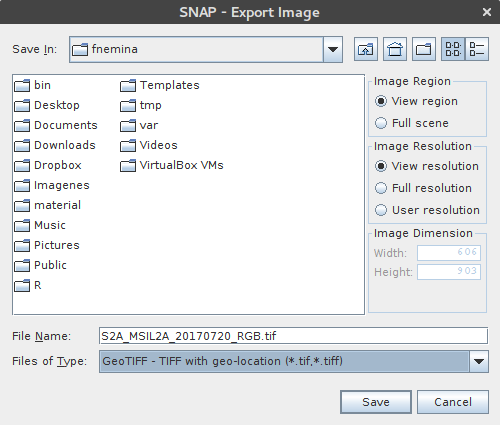
\includegraphics[width=0.7\textwidth]{fig:export.png}
    \caption{Menu de Export image. Incluye las opciones para elegir el recorte, la resolución y el tipo de dato de salida.}
    \label{fig:export}
\end{figure}

\section{Actividad}

Abra la imagen que se encuentra en la carpeta \directory{material/raster\_data>COSMO}. Abra la banda \path{Sigma0_VH}.

\begin{que}
    ¿A qué coberturas pertenecen las regiones de la imagen con mayor nivel de brillo?
\end{que}

\begin{que}
    ¿Cómo es el valor de brillo para los cuerpos de agua?
\end{que}

\begin{que}
    ¿Cuales son las coordenadas aproximadas del aeropuerto que se encuentra en el centro de la imagen?
\end{que}
